\documentclass[a4paper,12pt]{article}
\usepackage{xcolor}
\usepackage{algorithm}
\usepackage{algorithm}
\usepackage{algpseudocode}
\usepackage{amsmath,amsfonts,amssymb}
\usepackage{geometry}
\usepackage{fancyhdr}
\usepackage{graphicx}
\usepackage{caption}
\usepackage{titlesec}
\usepackage{tikz}
\usepackage{booktabs}
\usepackage{array}
\usetikzlibrary{positioning,arrows.meta} % Load the positioning library

\usetikzlibrary{shadows}
\usepackage{tcolorbox}
\usepackage{float}
\usepackage{lipsum}
\usepackage{mdframed}
\usepackage{pagecolor}
\usepackage{mathpazo}   % Palatino font (serif)
\usepackage{microtype}  % Better typography

% Page background color
\pagecolor{gray!10!white}

% Geometry settings
\geometry{margin=0.5in}
\pagestyle{fancy}
\fancyhf{}

% Fancy header and footer
\fancyhead[C]{\textbf{\color{blue!80}CS726 Programming Assignment -- 1 Report}}
\fancyhead[R]{\color{blue!80}Bayesian Bunch}
\fancyfoot[C]{\thepage}

% Custom Section Color and Format with Sans-serif font
\titleformat{\section}
{\sffamily\color{purple!90!black}\normalfont\Large\bfseries}
{\thesection}{1em}{}

% Custom subsection format
\titleformat{\subsection}
{\sffamily\color{cyan!80!black}\normalfont\large\bfseries}
{\thesubsection}{1em}{}

% Stylish Title with TikZ (Enhanced with gradient)
\newcommand{\cooltitle}[1]{%
  \begin{tikzpicture}
    \node[fill=blue!20,rounded corners=10pt,inner sep=12pt, drop shadow, top color=blue!50, bottom color=blue!30] (box)
    {\Huge \bfseries \color{black} #1};
  \end{tikzpicture}
}
\usepackage{float} % Add this package

\newenvironment{solution}[2][]{%
    \begin{mdframed}[linecolor=blue!70!black, linewidth=2pt, roundcorner=10pt, backgroundcolor=yellow!10!white, skipabove=12pt, skipbelow=12pt]%
        \textbf{\large #2}
        \par\noindent\rule{\textwidth}{0.4pt}
}{
    \end{mdframed}
}

% Document title
\title{\cooltitle{CS726 Programming Assignment -- 1 Report}}
\author{
\textbf{Saksham Rathi (22B1003)}\\
\textbf{Sharvanee Sonawane (22B0943)}\\
\textbf{Deeksha Dhiwakar (22B0988)}\\
\small Department of Computer Science, \\
Indian Institute of Technology Bombay \\}
\date{}

\begin{document}
\maketitle

\section{Triangulation}
This step is implemented in the function \texttt{triangulate}$\_$\texttt{and}$\_$\texttt{get}$\_$\texttt{cliques}. We first check if the graph is already triangulated, using the function \texttt{whether}$\_$\texttt{triangulated} described below:
\begin{algorithm}
\caption{Check if Graph is already Triangulated}
\begin{algorithmic}[1]

    \State \texttt{cycles} $\gets$ Find all cycles in graph

    \For{each \texttt{cycle} in \texttt{cycles}}
        \If{length of \texttt{cycle} $\ge$ 4}      

            \If{there is no shortcut (vertices connected by non-cycle edge)}                
                \State \textbf{return} False
            \EndIf
        \EndIf
    \EndFor

        \State \textbf{return} \texttt{True}
\end{algorithmic}
\end{algorithm}


If the graph is already triangulated, we directly proceed with extracting the maximal cliques. If the graph is not triangulated, we first triangulate it using the minimum degree heuristic, as described in the pseudocode below:

\begin{algorithm}
\caption{Triangulation Process}
\begin{algorithmic}[1]

    \State \texttt{vertices\_left} $\gets$ Set of all vertices



    \While{\texttt{vertices\_left} is not empty}
        \State \texttt{vertex} $\gets$ Vertex in \texttt{vertices\_left} with minimum degree

        \For{each pair $(i, j)$ of neighbours of \texttt{vertex}}
            \If{the graph does not contain an edge between $i$ and $j$}
                \State Add edge $(i, j)$ to the original graph
            \EndIf
        \EndFor
        \State Remove \texttt{vertex} from \texttt{vertices\_left}

        \State Update graph by removing \texttt{vertex} and updating degrees and edges
    \EndWhile
\end{algorithmic}
\end{algorithm}

The figure below shows the run of the triangulation algorithm on an example graph:

\begin{center}
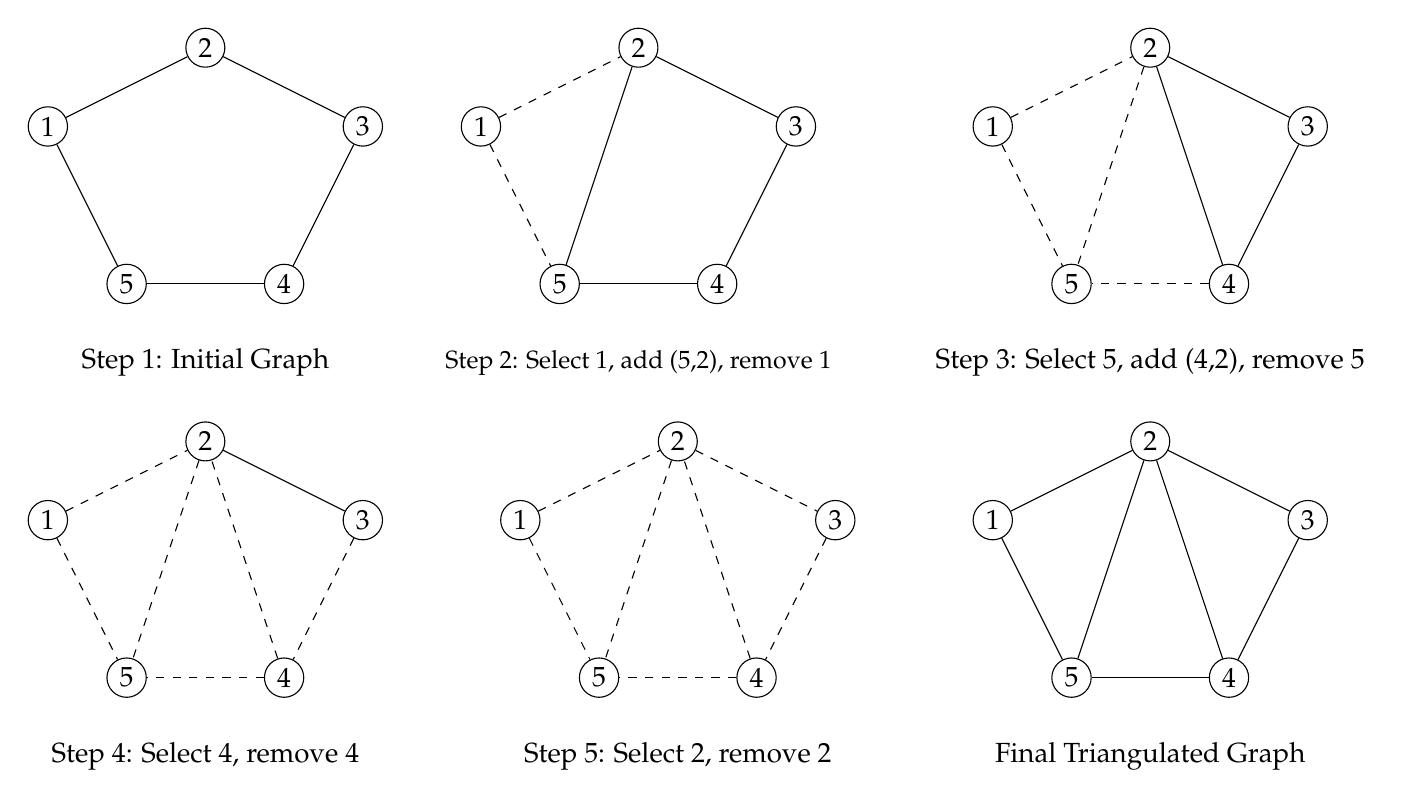
\begin{tikzpicture}[scale=1]

    % Step 1: Initial Graph (First row, first column)
    \begin{scope}
        \node[draw, circle, inner sep=2pt] (1) at (0,2) {1};
        \node[draw, circle, inner sep=2pt] (2) at (2,3) {2};
        \node[draw, circle, inner sep=2pt] (3) at (4,2) {3};
        \node[draw, circle, inner sep=2pt] (4) at (3,0) {4};
        \node[draw, circle, inner sep=2pt] (5) at (1,0) {5};

        \draw (1) -- (2);
        \draw (2) -- (3);
        \draw (3) -- (4);
        \draw (4) -- (5);
        \draw (5) -- (1);

        \node at (2,-1) {Step 1: Initial Graph};
    \end{scope}

    % Step 2: Pick vertex 1, connect 5-2, then remove 1 (First row, second column)
    \begin{scope}[xshift=5.5cm]
        \node[draw, circle, inner sep=2pt] (1b) at (0,2) {1};
        \node[draw, circle, inner sep=2pt] (2b) at (2,3) {2};
        \node[draw, circle, inner sep=2pt] (3b) at (4,2) {3};
        \node[draw, circle, inner sep=2pt] (4b) at (3,0) {4};
        \node[draw, circle, inner sep=2pt] (5b) at (1,0) {5};

        \draw (2b) -- (3b);
        \draw (3b) -- (4b);
        \draw (4b) -- (5b);
        \draw (5b) -- (2b);
        \draw[dashed] (1b) -- (2b); % Added edge
        \draw[dashed] (1b) -- (5b); % Added edge

        \node at (2,-1) {\small Step 2: Select 1, add (5,2), remove 1};
    \end{scope}

    % Step 3: Pick vertex 5, connect 4-2, then remove 5 (First row, third column)
    \begin{scope}[xshift=12cm]
        \node[draw, circle, inner sep=2pt] (1b) at (0,2) {1};
        \node[draw, circle, inner sep=2pt] (2b) at (2,3) {2};
        \node[draw, circle, inner sep=2pt] (3b) at (4,2) {3};
        \node[draw, circle, inner sep=2pt] (4b) at (3,0) {4};
        \node[draw, circle, inner sep=2pt] (5b) at (1,0) {5};

        \draw (2b) -- (3b);
        \draw (3b) -- (4b);
        
        \draw (4b) -- (2b);
        \draw[dashed] (1b) -- (2b); % Added edge
        \draw[dashed] (1b) -- (5b); % Added edge
        \draw[dashed] (4b) -- (5b); % Added edge
        \draw[dashed] (2b) -- (5b); % Added edge
        

        \node at (2,-1) {Step 3: Select 5, add (4,2), remove 5};
    \end{scope}

    % Step 4: Pick vertex 4, connect 3-2, then remove 4 (Second row, first column)
    \begin{scope}[yshift=-5cm]
        \node[draw, circle, inner sep=2pt] (1b) at (0,2) {1};
        \node[draw, circle, inner sep=2pt] (2b) at (2,3) {2};
        \node[draw, circle, inner sep=2pt] (3b) at (4,2) {3};
        \node[draw, circle, inner sep=2pt] (4b) at (3,0) {4};
        \node[draw, circle, inner sep=2pt] (5b) at (1,0) {5};

        \draw (2b) -- (3b);
        \draw[dashed] (3b) -- (4b);
        
        \draw[dashed] (4b) -- (2b);
        \draw[dashed] (1b) -- (2b); % Added edge
        \draw[dashed] (1b) -- (5b); % Added edge
        \draw[dashed] (4b) -- (5b); % Added edge
        \draw[dashed] (2b) -- (5b); % Added edge
        

        \node at (2,-1) {Step 4: Select 4, remove 4};
    \end{scope}

    % Step 5: Remove remaining vertices (Second row, second column)
    \begin{scope}[yshift=-5cm, xshift=6cm]
     \node[draw, circle, inner sep=2pt] (1b) at (0,2) {1};
        \node[draw, circle, inner sep=2pt] (2b) at (2,3) {2};
        \node[draw, circle, inner sep=2pt] (3b) at (4,2) {3};
        \node[draw, circle, inner sep=2pt] (4b) at (3,0) {4};
        \node[draw, circle, inner sep=2pt] (5b) at (1,0) {5};

        \draw[dashed] (2b) -- (3b);
        \draw[dashed] (3b) -- (4b);
        
        \draw[dashed] (4b) -- (2b);
        \draw[dashed] (1b) -- (2b); % Added edge
        \draw[dashed] (1b) -- (5b); % Added edge
        \draw[dashed] (4b) -- (5b); % Added edge
        \draw[dashed] (2b) -- (5b); % Added edge
        

        \node at (2,-1) {Step 5: Select 2, remove 2};

    \end{scope}

        \begin{scope}[yshift=-5cm, xshift=12cm]
     \node[draw, circle, inner sep=2pt] (1b) at (0,2) {1};
        \node[draw, circle, inner sep=2pt] (2b) at (2,3) {2};
        \node[draw, circle, inner sep=2pt] (3b) at (4,2) {3};
        \node[draw, circle, inner sep=2pt] (4b) at (3,0) {4};
        \node[draw, circle, inner sep=2pt] (5b) at (1,0) {5};

        \draw(2b) -- (3b);
        \draw (3b) -- (4b);
        
        \draw (4b) -- (2b);
        \draw (1b) -- (2b); % Added edge
        \draw (1b) -- (5b); % Added edge
        \draw (4b) -- (5b); % Added edge
        \draw (2b) -- (5b); % Added edge
        

        \node at (2,-1) {Final Triangulated Graph};

    \end{scope}

    

\end{tikzpicture}
\end{center}
    Once we obtain the triangulated graph, we extract the maximal cliques from it using the function \texttt{get\_maximal\_cliques}, which uses the Bron-Kerbosch algorithm described below:

\begin{algorithm}
\caption{Bron–Kerbosch Algorithm for Finding Maximal Cliques}
\begin{algorithmic}[1]
    \Procedure{Bron\_Kerbosch}{$\text{current\_clique}, \text{candidates}, \text{excluded}, \text{maximal\_cliques}$}
        \If{$\text{candidates}$ is empty \textbf{and} $\text{excluded}$ is empty} 
            \State Add $\text{current\_clique}$ to $\text{maximal\_cliques}$
            \State \Return
        \EndIf
        
        \For{each vertex $v$ in $\text{candidates}$}
            \State \texttt{Bron\_Kerbosch}($\text{current\_clique} \cup \{v\},$
            \State \hspace{1cm} $\text{candidates} \cap \text{Neighbors}(v),$
            \State \hspace{1cm} $\text{excluded} \cap \text{Neighbors}(v),$
            \State \hspace{1cm} $\text{maximal\_cliques}$)
            \State Remove $v$ from $\text{candidates}$
            \State Add $v$ to $\text{excluded}$
        \EndFor
    \EndProcedure
\end{algorithmic}
\end{algorithm}




















\section{Junction Tree Construction}
This step is implemented in the $\texttt{get\_junction\_tree}$ function. We use the maximal cliques obtained after the triangulation process to create the junction tree while maintaining the running intersection property. Each clique in this tree retains its assigned potential values.
\begin{algorithm}
\caption{Constructing a Junction Tree from Maximal Cliques}
\begin{algorithmic}[1]
\Require Set of maximal cliques $\mathcal{C}$
\Ensure Junction tree satisfying the running intersection property

\State Initialize an empty priority queue $T$
\ForAll{pairs $(C_1, C_2)$ in $\mathcal{C}$}
    \State Compute the intersection set $S = C_1 \cap C_2$
    \If{$S \neq \emptyset$}
        \State Compute weight $w = |S|$
        \State Push $(-w, C_1, C_2)$ onto $T$ (negative weight for max heap)
    \EndIf
\EndFor
\\
\State Initialize $parent[C] = C$ and $rank[C] = 0$ for all $C \in \mathcal{C}$
\\
\Function{FindParent}{$C$}
    \If{$parent[C] \neq C$}
        \State $parent[C] \gets \text{FindParent}(parent[C])$
    \EndIf
    \State \Return $parent[C]$
\EndFunction
\\
\Function{Union}{$C_1, C_2$}
    \State $root_1 \gets \text{FindParent}(C_1)$
    \State $root_2 \gets \text{FindParent}(C_2)$
    \If{$root_1 \neq root_2$}
        \If{$rank[root_1] > rank[root_2]$}
            \State $parent[root_2] \gets root_1$
        \ElsIf{$rank[root_2] > rank[root_1]$}
            \State $parent[root_1] \gets root_2$
        \Else
            \State $parent[root_2] \gets root_1$
            \State $rank[root_1] \gets rank[root_1] + 1$
        \EndIf
        \State \Return True
    \EndIf
    \State \Return False
\EndFunction
\\
\State Initialize an empty set $MST$ (Minimum Spanning Tree)
\While{$T$ is not empty}
    \State Pop $(w, C_1, C_2)$ from $T$
    \If{\Call{Union}{$C_1, C_2$}}
        \State Add edge $(C_1, C_2)$ to $MST$
    \EndIf
\EndWhile

\State \Return $MST$
\end{algorithmic}
\end{algorithm}
Consider the given triangulated graph:
\begin{center}
    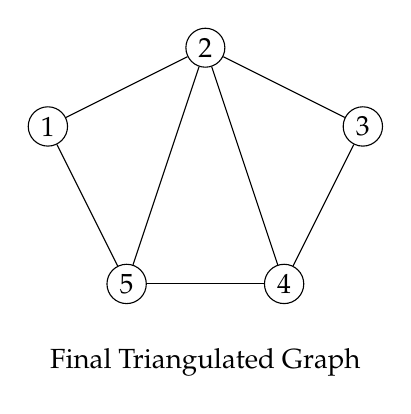
\begin{tikzpicture}
    \begin{scope}[yshift=-5cm, xshift=12cm]
     \node[draw, circle, inner sep=2pt] (1b) at (0,2) {1};
        \node[draw, circle, inner sep=2pt] (2b) at (2,3) {2};
        \node[draw, circle, inner sep=2pt] (3b) at (4,2) {3};
        \node[draw, circle, inner sep=2pt] (4b) at (3,0) {4};
        \node[draw, circle, inner sep=2pt] (5b) at (1,0) {5};

        \draw(2b) -- (3b);
        \draw (3b) -- (4b);
        \draw (4b) -- (2b);
        \draw (1b) -- (2b); 
        \draw (1b) -- (5b);
        \draw (4b) -- (5b);
        \draw (2b) -- (5b); 

        \node at (2,-1) {Final Triangulated Graph};
    \end{scope}
    \end{tikzpicture}
\end{center}
From the triangulated graph, we obtain the maximal cliques:
\[
C_1 = \{1,2,5\}, \quad
C_2 = \{2,3,4\}, \quad
C_3 = \{2,4,5\}, \quad
\]
The intersection sets are as follows: 
\begin{align*}
C_1 \cap C_3 &= \{2,5\}, \quad |C_1 \cap C_3| = 2 \\
C_1 \cap C_2 &= \{2\}, \quad |C_1 \cap C_2| = 1 \\
C_3 \cap C_2 &= \{2,4\}, \quad |C_3 \cap C_2| = 2 \\
\end{align*}
We construct edges with weights corresponding to intersection sizes:
\[
(C_1, C_3, 2), \quad (C_3, C_2, 2), \quad (C_1, C_2, 1)
\]
Using Kruskal’s algorithm:
\begin{enumerate}
    \item Sort edges: $(C_1, C_3, 2)$, $(C_3, C_2, 2)$, $(C_1, C_2, 1)$.
    \item Add $(C_1, C_3)$ (weight 2).
    \item Add $(C_3, C_2)$ (weight 2).
    \item Ignore $(C_1, C_2)$ (weight 1) as it would form a cycle.
\end{enumerate}
\textbf{Final Junction Tree:}
\[
C_1 \leftrightarrow C_3 \leftrightarrow C_2
\]
\begin{center}
    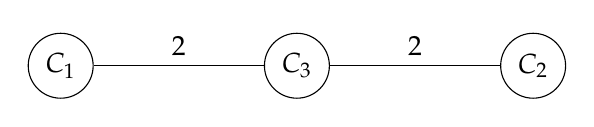
\begin{tikzpicture}
        \node[draw, circle] (C1) at (0,0) {$C_1$};
        \node[draw, circle] (C3) at (3,0) {$C_3$};
        \node[draw, circle] (C2) at (6,0) {$C_2$};

        \draw (C1) -- node[above] {2} (C3);
        \draw (C3) -- node[above] {2} (C2);
    \end{tikzpicture}
\end{center}
For any two cliques $C_i$ and $C_j$ containing the same variable $X$, all cliques along the unique path in the tree must contain $X$. This holds for all intersections.


\section{Marginal Probability}
Here is the pseudocode for sharing messages between the maximal cliques of the graph.

\subsection*{Computing the partition function}  
Firstly, we show how to calculate the Z value for the given graph. So, we first select a root node and then perform a depth-first search (DFS) to calculate the depth of each maximal clique (node in the junction tree). Then, we send messages from the deepest leaves till the root node. Finally, we calculate the partition function using the root clique potential and the received messages. (Messages are being sent again from root to the internal nodes and finally to the leaves, to be used in the next step of computing marginal probabilities.)    

\begin{algorithm}
    \caption{Computation of Partition Function \( Z \)}
    \begin{algorithmic}[1]
    \Require Graphical Model with maximal cliques and potentials
    \Ensure Partition function \( Z \)
    
    \State Construct the junction tree \( JT \) from maximal cliques
    \State Initialize adjacency list \( JT_{adj} \) from \( JT \)
    
    \State Select a root clique \( C_{root} \)
    \State Initialize depth map with \( C_{root} \) at depth 0
    
    \Function{DFS}{$node, parent, depth$}
        \For{each child in \( JT_{adj}[node] \)}
            \If{child $\neq$ parent}
                \State Update depth map
                \State Call DFS on child with depth $+1$
            \EndIf
        \EndFor
    \EndFunction
    
    \State Perform DFS from \( C_{root} \)
    
    \Function{SendMessage}{$C_{from}, C_{to}$}
        \State Compute separator set \( S = C_{from} \cap C_{to} \)
        \State Initialize message vector \( M \) of size \( 2^{|S|} \)
        \State Modify clique potential based on incoming messages
        \For{each state assignment in \( C_{from} \)}
            \State Compute corresponding separator index
            \State Aggregate message value
        \EndFor
        \State Store message \( M(C_{from} \to C_{to}) \)
    \EndFunction
    
    \State Initialize messages dictionary
    \State Initialize clique potentials
    
    \For{each clique from deepest to root}
        \State Send messages to parent cliques
    \EndFor
    
    \For{each clique from root to leaves}
        \State Send messages to child cliques
    \EndFor
    
    \State Compute partition function \( Z \) using root clique potential and received messages
    \State \Return \( Z \)
    
    \end{algorithmic}
\end{algorithm}

\subsection*{Computing the marginal probabilities}
Here is the pseudocode for computing the marginal probabilities in the graphical model using message passing. We get the partition function \( Z \) from the previous step and use it to normalize the marginal probabilities. We iterate over each variable in the graphical model and find the maximal clique containing it. We then extract the potential function for the clique (using the messages received from neighboring cliques) and compute the marginal probability for the variable. (For every variable, we need to do this only for one clique containing it, as the marginal probability will be the same in all maximal cliques containing the variable.)


\begin{algorithm}
    \caption{Computation of Marginal Probabilities}
    \begin{algorithmic}[1]
    \Require Graphical Model with maximal cliques, clique potentials, and messages
    \Ensure Marginal probabilities for each variable

    \State Initialize adjacency list for junction tree
    \State Retrieve partition function $Z$ using previously computed values
    \State Initialize marginal probability list $M$ with zeros

    \For{each variable $X_i$ in the graphical model}
        \State Find a maximal clique $C$ containing $X_i$
        \State Extract the potential function for clique $C$

        \For{each neighboring clique $C'$ of $C$}
            \State Compute separator set $S = C \cap C'$
            \State Retrieve message $M(C' \to C)$
            \For{each assignment in $C$}
                \State Identify corresponding index in $S$
                \State Multiply message values with clique potential
            \EndFor
        \EndFor

        \State Compute marginal probability for $X_i$
        \State Normalize values using $Z$
    \EndFor

    \State \Return $M$
    \end{algorithmic}
\end{algorithm}




\section{Finding the Most Probable Assignment}
Here is the pseudocode for finding the top-K most probable assignments in the graphical model. The value of the partition function \( Z \) is used from the previous step. Similar to the previous step, we do a DFS to calculate the depth of each maximal clique. We then send messages from the deepest leaves to the root node. This time the messages which are being send are of a different format, and they contain the following two values:
\begin{itemize}
    \item The union of all sets of variables seen so far (from its descendants and including itself).
    \item Mapping between the assignments of the variables in the union set, and the corresponding product of potentials.
\end{itemize}

{\bf Optimization Step:} We maintain a set of extra variables, which are present in the clique from which a message is sent as compared to the clique to which the message is being sent. For all possible assignments of the extra variables, we only pick the top-K assignments for all other variables. This optimizes the algorithm by reducing the number of assignments being sent in the message.

Finally, we send a message from the root node to ``None'', which basically collects the assignments of all the variables in the graphical model. We then normalize the probabilities and return the top-K most probable assignments.


\begin{algorithm}
    \caption{Compute Top-K Assignments in Graphical Model}
    \begin{algorithmic}[1]
    \State \textbf{Input:} Graphical model with junction tree, clique potentials, $k$ value
    \State \textbf{Output:} Top-$k$ assignments with highest probabilities
    
    \State $junction\_tree \gets$ get the junction tree
    \State Initialize $junction\_tree\_adj\_list$ as empty dictionary
    \For{each edge $(a, b)$ in $junction\_tree$}
    \State Add $b$ to adjacency list of $a$ and vice versa
    \EndFor
    
    \State $root \gets$ any maximal clique as the root
    \State Initialize $depth\_map$ with $root$ having depth $0$
    \Procedure{DFS}{$node, parent, depth$}
    \For{each child in adjacency list of $node$}
    \If{child $\neq$ parent}
    \State Set depth of $child$ and call DFS recursively
    \EndIf
    \EndFor
    \EndProcedure
    \State Call DFS($root, \text{None}, 1$)
    
    \Procedure{SendMessage}{$from\_clique, to\_clique, parent\_map, clique\_potentials, messages$}
    \State Compute variables seen and neighboring variables
    \State Initialize message with uniform probability distribution
    \For{each assignment in possible values of seen variables}
    \State Compute potential index and update probability
    \State Multiply with incoming messages from neighboring cliques
    \EndFor
    \State {\textit{\bf For each of the extra variables in the current clique (as compared to the clique to which we are sending the message, we pick only the top-K assignments for all other variables, this is essentially the optimization of the algorithm)}}
    \State Store the computed message in $messages$
    \EndProcedure
    
    \State Initialize $messages$ as an empty dictionary
    \State $clique\_potentials \gets$ get clique potentials
    \State $max\_depth \gets$ maximum depth in $depth\_map$
    
    \For{$depth = max\_depth$ down to $0$}
    \For{each clique at depth $depth$}
    \State Identify parent cliques
    \For{each parent clique}
    \State Call SendMessage with $(clique, parent, ...)$
    \EndFor
    \EndFor
    \EndFor
    
    \State Call SendMessage with $(root, \text{None}, ...)$
    \State $message\_final \gets$ computed message from root
    \State Normalize probabilities using partition function $Z$
    
    \State Sort assignments by probability in descending order
    \State Return top-$k$ assignments
    
    \end{algorithmic}
    \end{algorithm}


\end{document}
